\documentclass{fisatproject}
\usepackage{graphicx}
\title{Website Design Ranking Using ML}
\team{Adhyaksh Guhan \\ Anet Eliza Johny\\ Dharwish Raj \\ Joel J Padayattil}
\author{Dharwish Raj}
\begin{document}
\maketitle

\makecert

\newpage
%\thispagestyle{plain}
\pagenumbering{roman}
\setcounter{page}{1}
\newgeometry{top=4cm,bottom=0.1cm}
\renewcommand\abstractname{ABSTRACT}
\begin{abstract}
\vspace{5cm}
This project attempts to review and rank websites objectively and without any human input. Most website design rankings,if not all, are subjective in nature and curated by human hands and minds.Website Design Ranker attempt to achieve similar results but with computer algorithms for a fairer comparison.

Website design ranking is usually done by a committee of experts or by mass voting on the internet. This method of ranking can be unfavorable due to the subjectivity of its nature.There are no clear standards on which everyone can definitely agree on and it causes the whole process to be an unfair popularity contest.This project,with its lack of human input and unbiased perspective can be used as an objective basis from where ranking can commence.

Currently,the ranking of the designs are done by the counting of the number of colours contained in a website. This is done by using a web scrapper to scrap the website and obtain the CSS file. The file is then parsed through using a regex method, and is used to find and count hexcodes contained within. The resulting number is then printed and then used as a parameter to rank-based on colour theory-if the website has too few colours or too many colours or if it has just the right amount.
\end{abstract}


\newpage
%\thispagestyle{plain}
\renewcommand\abstractname{ACKNOWLEDGMENT}
\begin{abstract}
\vspace{5cm}
If words are considered as symbols of approval and tokens of acknowledgement, then let the words play the heralding role of expressing our gratitude. Firstly, we praise the God Almighty for the grace he showered on us during our studies as well as our daily activities.

We thank our Principal,\textbf{Dr. George Issac}, for the amenities provided,which helped us in the fullfillment of our project. We would also thank our beloved \textbf{Dr. Prasad J.C. (H.O.D)} who helped in all the phases of our project.

We pay our gratitude to all project staff in-charges, \textbf{Ms. Soumya S. Raj, Mr. Anuranj P., Ms. Simi Stephen} for their constant support and encouragement for the project. We are extremely thankful to our project guide \textbf{Mr. Pankaj Kumar}, who always helped and guided for all the success of our project.

We express our sincere gratitude to all faculties of Computer Science Department, \textbf{FISAT}. We also thank our parents and friends for supporting in the completion of our project.
\vspace{1cm}
\begin{flushright}
Adhyaksh Guhan

Anet Eliza Johny

Dharwish Raj

Joel J Padayattil
\end{flushright}
\end{abstract}
\newpage

\restoregeometry
\tableofcontents
\newpage

\cleardoublepage
\addcontentsline{toc}{chapter}{\listfigurename}
\listoffigures
\newpage

\cleardoublepage
\addcontentsline{toc}{chapter}{\listtablename}
\listoftables
\newpage
\pagestyle{fancy}


\chapter{INTRODUCTION}
\pagenumbering{arabic}
\setcounter{page}{1}
\renewcommand{\baselinestretch}{1.50}
\section{Overview}
The website design is an important factor in the growth of that website. It makes a difference on how the target audience view the business or company.So website design ranking is important for the audience to choose the best website.Recently this ranking is done manually by looking into the websites by a group of people.

Ranking of website design manually is a difficult and time consuming method. Website Design Ranker can overcome this difficulty by automating the ranking mechanism. Since a perfect model for website ranking is not in practice this follows ranking according to submissions by critics. Website Design Ranker reduces the difficulty and increases the accuracy in ranking since it is using an algorithm for ranking.

Website Design Ranker will rank set of input websites based
on certain parameters.Too many colors can create a sense of confusion. As colour is an important factor to attract as well as repel the audience of a website. So the Website Design Ranker uses colour as a parameter to rank different websites accordingly.
\section{Scope of Project}
There was no existing methodology for analyzing and evaluating website designs. The method which followed until this time was based on submissions by the critics. This method can be replaced by our automated system to rank website design based on the different parameters, say colour,grid etc.
\chapter{RELATED WORK}
\section{Google Page Layout Algorithm}
Google introduced Page Layout Algorithm to analyze website
readability.[1] It looks for the layout of the web page and the amount of
content we see in the page once we click on a result.[1] It focuses to reduce the difficulty of users to find the actual
content.[1]
The websites which does not have a lot of visible content
above-the-fold and dedicates a large fraction (above a normal
degree) to ads, will be affected.[1]


\begin{figure}

	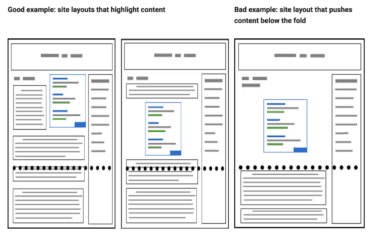
\includegraphics[width=10cm]{image/gpa.png}
	\caption{One of the criteria of GPL Algorithm\textsuperscript{[Fig:1]}}
	\label{fig1:gpa}

\end{figure}


Determine the old design of the website.If a website has many advertisements above the fold(the part of page that is visible on the screen when the page first loads before scrolling)then it is considered as the first drawback.Else if a website has a large flash animations or other
non-content elements that forces users to scroll to see the content, then that will be the next drawback. If there is specific amount of ads and content of website required for audience, there will be no drawback.These drawbacks will affect the ranking process. If these conditions are met the website ranks a low rank. Else its rank will be considerabily high.




\chapter{DESIGN and IMPLEMENTATION}

\section{Design}
Website Design Ranker will rank set of input websites based
on certain parameters.
The parameters we are focussing on are color and grid .
Then we move on for public review.
This will be helpful in finding the best website among list of
websites.
The website design can be compared with other competing
websites.
This show a  website’s design may improve in an area.


\subsection{Algorithm}
\begin{itemize}
	\item[1.] Start.
	\item[2.] Using a website scraper to accept the various website
	addresses.
	\item[3.] Scraping through the source code of each website via CSS files.
	\item[4.] Find the hex codes of all elements of the website and count them with a count variable.
	\item[5.] If count == 0 then give mark as 0.
	\item[6.] else if count is greater than or equal to 5, then also give mark as 0.
	\item[7.]If the count is less than or equal to 5,then the mark provided will be 1.
	\item[8.]Stop.
\end{itemize}
\subsection{System Requirements}
\subsubsection{\underline{Software Requirements}}
\begin{itemize}
	\item Operating System : LINUX OS 
	
	\item Language : Python Language
\end{itemize}

\subsubsection{\underline{Hardware Requirements}}
\begin{itemize}
	\item Processor : Intel core i3, i5 
	\item RAM : 8 GB
	\item Hard Disk : 1 TB
	
\end{itemize}

\section{Implementation}
\subsection{Data Flow Diagram - Level 0}
\begin{flushleft}
	\centerline{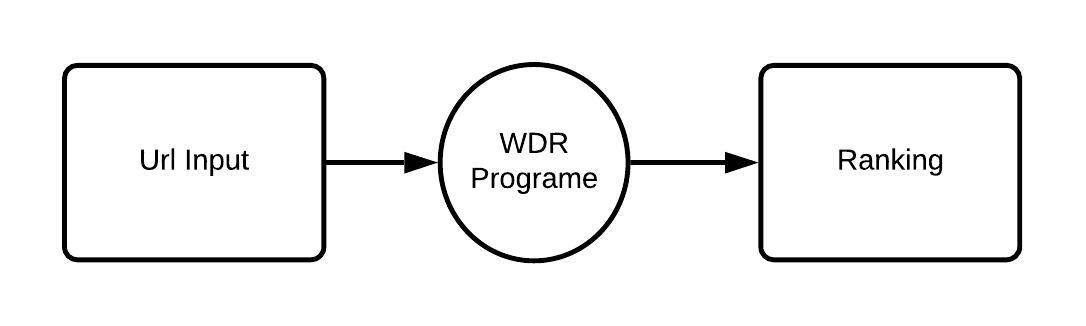
\includegraphics[scale=1.2]{image/level_0_dfd.jpeg}}
\end{flushleft}
\subsection{Data Flow Diagram - Level 1}
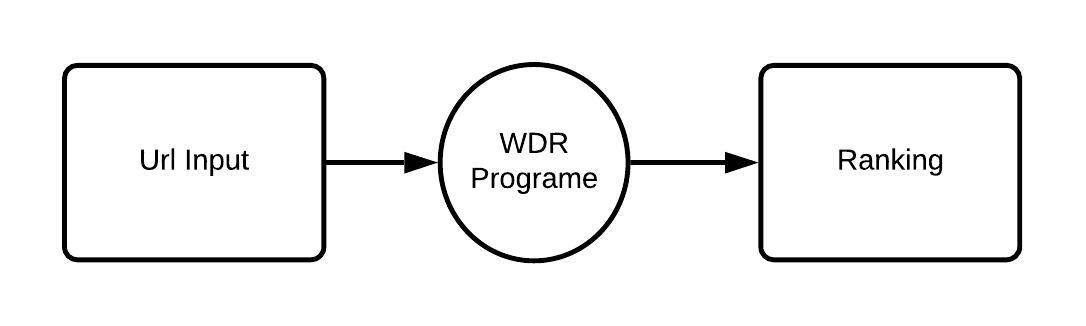
\includegraphics[scale=0.80]{image/level_0_dfd.jpeg}
\newpage
On the basis of colour theory, we count the number of
colours to determine the ranking of the website.
Too few colours, then the website is extremely simple and too
boring.
Too many colours, then the website is over-designed and busy.
The system works by scrapping CSS file of different websites using webscrapper and from that CSS files it find and count the hexcodes of websites using regular expression.This count is used to rank the websites accordingly.Websites with too many and too few colours are ranked less and those with a specific count of colours are ranked high.    
\chapter{TESTING}

	Testing was done in several stages of this project. It was helpful to determine suitable language and library to collect data from different websites to find out ranking\\
	\subsection{Scrapping CSS codes from websites}
\begin{itemize}
	\item A website template's 'style.css' file was downloaded and then used as subject to testing the colour counting code.
	\item A website was created to have public ranking of various websites with a possible ranking of 1-5 (1 being the lowest, 5 the highest). This could then be used as ranking data for the program.
\end{itemize}
\chapter{RESULTS}
	\begin{itemize}
		\item Number of colours counted:
	\begin{figure}[h]
		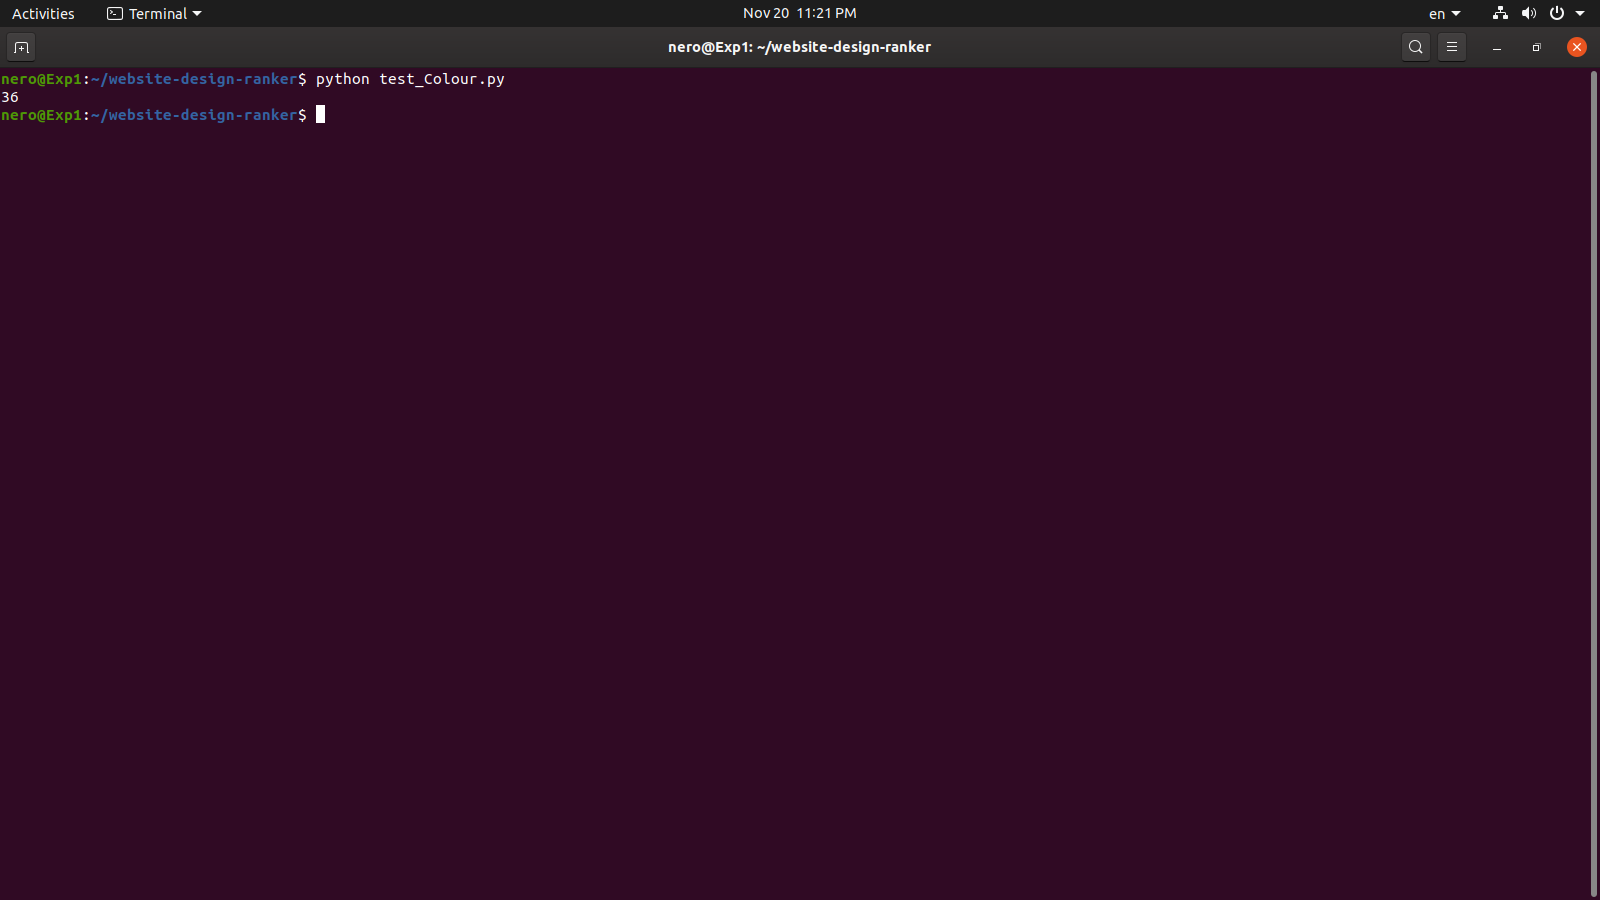
\includegraphics[scale=.3]{colourtest.png}
	\end{figure}
	\end{itemize}
Compiled languages are languages typically processed by compilers, though theoretically any language can be compiled or interpreted. The important ones are:
\begin{itemize}
\item Ada
\item C
\item C++
\item Fortran
\item Java
\end{itemize}

\chapter{CONTRIBUTIONS}
\begin{itemize}
	\item Dharwish Raj - Creation of website for public ranking and code correction
	\item Adhyaksh Guhan - Creation of code for colour counting and spell checking
	\item Joel J Padayattil - Creation of UI using PyQT5
	\item Anet Eliza Johny - Proposed and Implemented basic algorithm 
\end{itemize}
\chapter{CONCLUSION}

A Website Design Ranker is an automated method to rank websites based on their design by comparing certain parameters. Here we can see the logical differences in the approaches that our algorithm takes versus any existing methods.To make ranking easier, the Website Design Ranker uses an algorithm to rank websites based on parameter colour.

Nowadays, ranking websites is done manually by a committee or a group of people. To avoid or to reduce the human involvement, Website Design Ranker is a suitable method. In this report, we have discussed our approach to rank a website design.



\begin{thebibliography}{1}
\bibitem{nist} Google Page Layout Algorithm: Everything You Need to
Know
 \url{https://www.searchenginejournal.com/google-algorithm-history/page-layout/close}

\end{thebibliography}

\begin{appendices}
\chapter{Sample Code}
\begin{lstlisting}[language=python]
	import re
	with open('style.css') as f:
	file\_contents = f.read()
	regex = r':?.(\#[0-9a-fA-F]\{6\}|\#[0-9a-fA-F]\{3\})'
	result = re.findall(regex, file\_contents)
	print(len(set(result)))

\end{lstlisting}
\end{appendices}


\end{document}
